\documentclass[12pt]{beamer}
\beamertemplatenavigationsymbolsempty

\usetheme{Copenhagen}
\useoutertheme{infolines}

\usepackage[utf8]{inputenc}
\usepackage[ngerman]{babel}
\usepackage{graphicx}
\usepackage{subfigure}
\title[Task5]{Task 5 \\Genetische Multipopulationsalgorithmen}
\institute{EvoTest}
\author{Alex, Yaroslav, Manuel}
\date{18.01.2017}

\begin{document}
\maketitle

\section{Einleitendes}
\frame{\frametitle{Ausgangssituation}
\begin{itemize}
\item Testframework für automatische Parksimulation wurde implementiert
\item Testfälle wurden mit Einsatz vom einfachen genetischen Algorithmus erzeugt
\item Eingrenzung auf eine Population führte zur hohen Homogenität der Testfälle

Das Ergebnis soll mit Hilfe von mehreren Population verbessert werden
\end{itemize}
}

\section{Aufgabe}
\frame{\frametitle{Aufgabe}
\begin{itemize}
\item  Erweiterung vom genetischen Algorithmus um mehrere Populationen
\item Umsetzung der drei Migrationsarten: ring, unrestricted, neighbour
\item Bewertung der MPGA Implementierung und Vergleich zum einfachen GA Ansatz
\end{itemize}
}

\section{Vorgehen}
\frame{\frametitle{Erzeugung der Populationen}
\begin{itemize}
\item Definition der Äquivalenzklassen als analytisch sinnvolle Testfälle 
\item Je Testfallklasse eine eigene Population mit zugewiesener Fitnessfunktion erzeugt welche Testfälle gewisser Art präferiert bzw. höher bewertet
\end{itemize}

}

\frame{\frametitle{Äquivalenzklassen}

\begin{itemize}
\item Äquivalenzklassen der angestrebten Testfälle wurden als Kombination vom Fahrzeug in Verhältnis zu Parklücke (links, rechts) sowie von Ausrichtung des Fahrzeugs (nach oben/unten, nach links/rechts) ermittelt
 
\item Für jede Variante wurde eine eigene Fitnessfunktion verwendet, die die gewünschte Fahrzeugposition und Ausrichtung bevorzugt

\end{itemize}
}

\frame{\frametitle{MPGA-Ansatz}
\begin{itemize}
\item 8 Populationen
\item Migrationsrate: 1 Chromosome je Migrationsvorgang und Population
\item Migrationsintervall: 20 Epochen
\item Anzahl Migrationsvorgänge: 20
\end{itemize}
}

\frame{\frametitle{Ring Migration Policy}
\begin{itemize}
\item Populationen logisch im Kreis angeordnet
\item Migration nur im Uhrzeigersinn möglich
\item Chromosom zur Migration wird zufällig in der Donor-Population ausgewählt
\item Die zu migrierende Chromosom wird dupliziert und ersetzt die Chromosom mit schlechtester Fitness in der Zielpopulation

\end{itemize}
}
\frame{\frametitle{Unrestricted Migration Policy}
\begin{itemize}
\item Migration aus allen restlichen Populationen möglich
\item Je Population wird ein Migrationspool mit fittesten Chromosomen aus den restlichen Populationen erzeugt
\item Eine Chromosom wird zufällig aus dem Pool ausgewählt und in die Empfängerpopulation migriert
\end{itemize}
}
\frame{\frametitle{Neighbour Migration Policy}
\begin{itemize}
\item Migrationspool wird nur aus Nachbarpopulationen erzeugt
\item Migrationslogik analog zu unrestricted policy
\end{itemize}
}

\section{Ergebnisse}
\frame{\frametitle{Ergebnisse: einfacher GA}
\centering
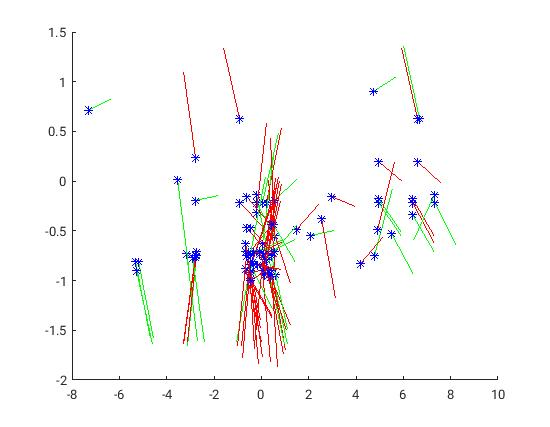
\includegraphics[width=.8\textwidth]{testcases_100chr_500epochs.jpg}
}
\frame{\frametitle{Ergebnisse MPFA: ohne Migration}
\centering
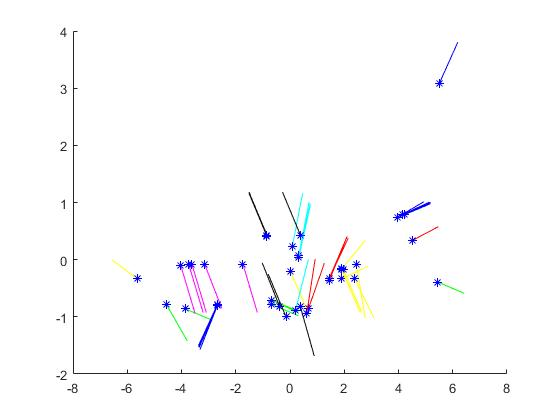
\includegraphics[width=.8\textwidth]{mpga_nomigration.jpg}
}
\frame{\frametitle{Ergebnisse MPGA: Ring Migration Policy}
\centering
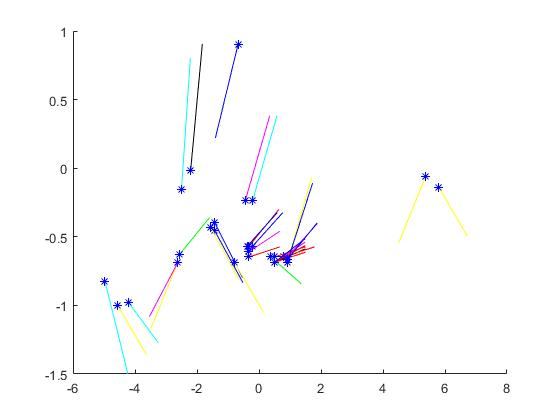
\includegraphics[width=.8\textwidth]{mpga_ring.jpg}
}
\frame{\frametitle{Ergebnisse MPGA: Unrestricted Migration Policy}
\centering
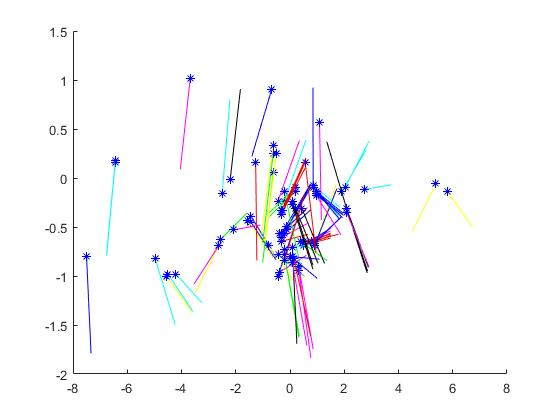
\includegraphics[width=.8\textwidth]{mpga_unrestricted.jpg}
}
\frame{\frametitle{Ergebnisse MPGA: Neighbour Migration Policy}
\centering
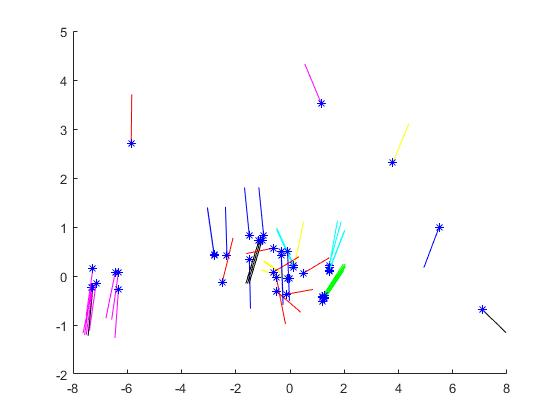
\includegraphics[width=.8\textwidth]{mpga_neighbour.jpg}
}
\frame{\frametitle{Analyse der Ergebnisse}
\begin{itemize}
\item Bedeutender Zuwachs an Heterogenität der Testfälle gegenüber den Ergebnissen vom einfachen genetischen Algorithmus
\item Konvergenz der Testfalleingenschaften innerhalb Populationen variiert je nach Migrationsmethode.
\item Selektionsdruck sowie Evolutionsrichtung können durch Fitnessfunktionen wirksam gesteuert werden

\end{itemize}
}

\section{Probleme und Ausblick}
\frame{\frametitle{Ausblick}
\begin{itemize}
\item Sensitivitätsanalyse mittels MPGA Parameter (Migrationsrate, Migration policy etc)
\item Ausarbeitung und Verfeinerung der einzelnen Fitnessfunktionen zur besseren Steuerung vom Selektionsdruck
\end{itemize}

}
\end{document}